\documentclass[12pt]{article}
\usepackage[utf8]{inputenc}
\usepackage[brazil]{babel}
\usepackage{amsmath, amsgen, amstext, amsbsy, amsopn, amsfonts, hyperref,  url, graphicx, tabularx, array, geometry, color}

\pagestyle{plain}

\setlength{\parskip}{1ex}
\setlength{\parindent}{0pt}

\renewcommand{\title}[1]{\textbf{#1}\\}
\renewcommand{\line}{\begin{tabularx}{\textwidth}{X>{\raggedleft}X}\hline\\\end{tabularx}\\[-0.5cm]}
\newcommand{\leftright}[2]{\begin{tabularx}{\textwidth}{X>{\raggedleft}X}#1%
& #2\\\end{tabularx}\\[-0.5cm]}


\begin{document}

\title{Oficina de Processing [at] Tarrafa Hackerspace}
\line
\leftright{\today}{Lucas Tonussi}

\section{Conhecendo Processing}

\qquad Processing foi desenvolvido por Casey Reas e Ben Fry com a idéia de que programação fosse descomplicada de se ensinar. Mas a comunicade do software livre/aberto viram que ele é uma ferramenta de manipulação gráfica muito poderosa. Processing é plataforma-múltipla por ser embarcada na Máquina Virtual Java, na verdade Processing é Java. Processing tem um sistema de arquivos próprio chamado Processing Developing Enviroment (extenção .pde) ou seja Processing tem sua própria IDE (lugar onde vai o programa, código).

\subsection{Agarre o Processing pra você!}

\qquad Visite \href{http://processing.org/download/}{Processing.org/download/} e selecione a versão que é \begin{Large}\textbf{compatível}\end{Large} com seu sistema operacional.

\qquad Veja:
\begin{itemize}
\item Qual arquitetura seu sistema operacional comporta: 32 bits ou 64 bits.
\item Qual é seu sistema operacional: Mac, Windows, ou Linux.
\item Faça o download da versão compatível.
\end{itemize}

\section{Abordando Processing}

\qquad Programar em Processing é bastante fácil, basta começar. No site do processing.org tem tudo quanto é tutorial e um fórum muito ativo esses docs tem muitas coisas tiradas de lá. Pois bem vamos começar com prática, por que sem praticar não tem como um dia começar a desenhar coisas bem mais bonitas e elaboradas, experiência própria. Ok Então vá ao \href{https://github.com/tonussi/oficinas/}{repo dessa oficina} e baixe o zip desse repositório, que contém todos os códigos que iremos trabalhar. E também todos os docs em \LaTeX. Essa oficina tem base nesses docs, utilizem para se guiarem durante a oficina. Sigam os passos e façam os exercícios.Processing BOOKS

\subsection{Exercício 1}

\qquad Para começarmos vamos com o básico. E o básico é entender o sistema de coordenadas e como ele funciona em Processing.

\begin{center}
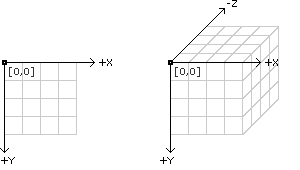
\includegraphics[scale=0.7]{coordinates}
\end{center}

\qquad Crie um novo sketch e faça o código seguinte, analisando nada linha. A Primeira você cria um plano, esse plano em Java é trabalhado para que você não precise se preocupar em como seu JPanel, FlowLayout, e BorderLayout irão ficar e como configurá-los. Tudo vem bem amarrado, basta que você desenhe. Para verificar o que eu estou dizendo digite, println(this); dentro de setup e você verá que tudo já vem construído. Ou seja a parte da programação em Java mais chata já vem pronta.

\begin{verbatim}
size(200, 200); //Cria o tamanho do seu plano
background(255); //Da cor para o fundo
noStroke(); //Tira o contorno
fill(255, 204, 0); //Preenche com cor
rect(30, 20, 50, 50); //Desenha um retângulo
\end{verbatim}

\subsection{Exercício 2}

\qquad \begin{verbatim}
void setup() {
  size(200, 200);
  noStroke();
  background(255);
  fill(0, 102, 153, 204);
  smooth();
  noLoop();
}

void draw() {
  circles(40, 80);
  circles(90, 70);
}

void circles(int x, int y) {
  ellipse(x, y, 50, 50);
  ellipse(x+20, y+20, 60, 60);
}
\end{verbatim}

\subsection{Exercício 3}

\qquad \begin{verbatim}
void setup() {
  size(200, 200);
  rectMode(CENTER);
  noStroke();
  fill(0, 102, 153, 204);
}

void draw() {
  background(255);
  rect(width-mouseX, height-mouseY, 50, 50);
  rect(mouseX, mouseY, 50, 50);
}
\end{verbatim}

\subsection{Execício 4}

\begin{verbatim}
size(200,200);
rectMode(CENTER);
rect(100,100,20,100);
ellipse(100,70,60,60);
ellipse(81,70,16,32);
ellipse(119,70,16,32);
line(90,150,80,160);
line(110,150,120,160);
\end{verbatim}

\end{document}
